\documentclass[tikz,border=2pt]{standalone}
\usepackage{tikz}
\usetikzlibrary{positioning}
\begin{document}
% Namikawa--Ueno type: III-I^*_l-t
% Target MRNC type: III-I^*_l-t
% Adapted from Tim Dokchitser picture: I^*_{{\it n}}\e({\it m})III
% Parameter substitution: n -> l, m -> t
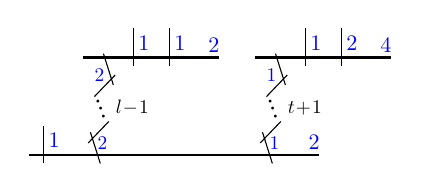
\begin{tikzpicture}[xscale=0.57,yscale=0.62]
\draw[thick,shorten >=2] (-1/3,0)--(94/15,0) node[inner sep=2pt,blue,above left,scale=0.8] {2};
\draw[shorten <=-3pt] (0,0)--node[inner sep=2pt,scale=0.8,blue,right] {1} (0,3/5);
\draw (6/5,0) 
    ++(0.06,-0.17)--++(-0.22,0.64)++(0.11,-0.24)  
    ++(0,0.02)
      node[blue,scale=0.7,inner sep=1,anchor=west]{2}
    ++(0,-0.02)
    ++(-0.16,0.02)--++(0.46,0.44)++(-0.12,0.08)  
    node{$\cdot$} ++(-0.06,0.16) node{$\cdot$}
    ++(-0.06,0.16) node{$\cdot$}++(0.17,-0.12)    node[auto,inner sep=5,scale=0.7,anchor=west]{$l\!-\!1$}
    ++(-0.25,0.23)--++(0.46,0.44)++(-0.19,0.04)   
    ++(0,-0.05)
      node[blue,scale=0.7,inner sep=1,anchor=east]{2}
    ++(0,0.05)
    ++(0.19,-0.04)++(-0.04,-0.2)--++(-0.22,0.64);
\draw[thick,shorten >=2] (13/15,2)--(121/30,2) node[inner sep=2pt,blue,above left,scale=0.8] {2};
\draw[shorten <=-3pt] (2,2)--node[inner sep=2pt,scale=0.8,blue,right] {1} (2,13/5);
\draw[shorten <=-3pt] (14/5,2)--node[inner sep=2pt,scale=0.8,blue,right] {1} (14/5,13/5);
\draw (151/30,0) 
    ++(0.06,-0.17)--++(-0.22,0.64)++(0.11,-0.24)  
    ++(0,0.02)
      node[blue,scale=0.7,inner sep=1,anchor=west]{1}
    ++(0,-0.02)
    ++(-0.16,0.02)--++(0.46,0.44)++(-0.12,0.08)  
    node{$\cdot$} ++(-0.06,0.16) node{$\cdot$}
    ++(-0.06,0.16) node{$\cdot$}++(0.17,-0.12)    node[auto,inner sep=5,scale=0.7,anchor=west]{$t\!+\!1$}
    ++(-0.25,0.23)--++(0.46,0.44)++(-0.19,0.04)   
    ++(0,-0.05)
      node[blue,scale=0.7,inner sep=1,anchor=east]{1}
    ++(0,0.05)
    ++(0.19,-0.04)++(-0.04,-0.2)--++(-0.22,0.64);
\draw[thick,shorten >=2] (47/10,2)--(118/15,2) node[inner sep=2pt,blue,above left,scale=0.8] {4};
\draw[shorten <=-3pt] (35/6,2)--node[inner sep=2pt,scale=0.8,blue,right] {1} (35/6,13/5);
\draw[shorten <=-3pt] (199/30,2)--node[inner sep=2pt,scale=0.8,blue,right] {2} (199/30,13/5);
\end{tikzpicture}
\end{document}
